\documentclass[12pt,a4paper]{report}

\renewcommand{\familydefault}{\sfdefault}

\usepackage[pdftex]{graphicx}
\usepackage{float}
\usepackage{fancyvrb}
\usepackage{minted}
\usepackage[utf8]{inputenc}
\usepackage[portuges]{babel}
\usepackage[T1]{fontenc}
\usepackage{times}
\usepackage[left=30mm,right=25mm,top=30mm,bottom=25mm,headsep=1.3cm]{geometry}
\usepackage{titlesec}
\usepackage{mathtools}
\graphicspath{{Imagens/}}
\usepackage{pdflscape}
\usepackage{indentfirst}
\usepackage{enumerate}
\usepackage{amsfonts}
\usepackage{fancyhdr}
\usepackage{amsfonts}
\usepackage{enumitem}
\usepackage{tabu}
\usepackage{float}
\usepackage{multicol}
\usepackage[table,xcdraw]{xcolor}
\usepackage{subfigure}
\usepackage{cite}
\usepackage{url}
\usepackage{hyperref}
\usepackage{enumitem}
\titlespacing*{\chapter}{0pt}{-0pt}{30pt}

\fancypagestyle{plain}{}
\pagestyle{fancy}
%\fancyhead[L]{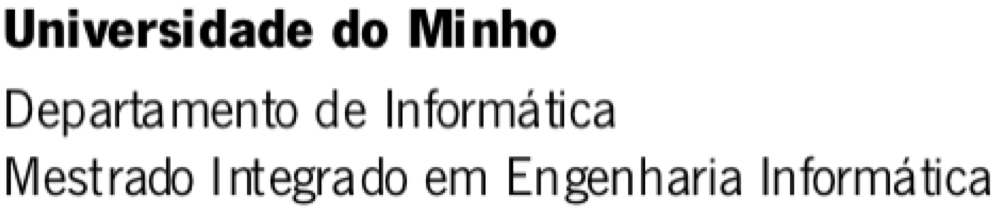
\includegraphics[scale=0.4]{Imagens/logoPB.png}}
\fancyhead[R]{Sistemas Emocionais em Programação de Robots\\ SI - Sistemas Autónomos}

\AtBeginEnvironment{minted}{\fontsize{11}{11}\selectfont}

\newcommand{\HRule}{\rule{\linewidth}{0.5mm}}
\titleformat{\chapter}{\bfseries\huge}{\thechapter.}{20pt}{\huge}


\begin{document}

\begin{titlepage}

\newgeometry{left=5cm,top=0cm}

\begin{minipage}{0.6\textwidth}
\begin{flushleft} 

\includegraphics[width=\textwidth]{./Imagens/logo.png}
\end{flushleft}
\end{minipage}

\vspace{3cm}

\Huge
\textbf{SI - Sistemas Autónomos\\}

\huge
\textit{Sistemas Emocionais em}

\textit{Programação de Robots}



\vfill
\normalsize

André Gonçalves, A75625

Miguel Miranda, A74726

Rogério Moreira, A74634

Tiago Sá, A71835

\vfill
Braga, {\today}

\end{titlepage}
\restoregeometry
\tableofcontents

\chapter{Introdução}

Redes neuronais artificias apresentam-se como um sistema conexionista, fortemente inspirado nas características do sistema nervoso central do ser humano. 
Apesar das RNAs serem um modelo simplificado, a sua arquitetura extremamente interligada de unidades de processamento permite que estas sejam capazes de generalizar e adquirir conhecimento, através de um processo de aprendizagem. 

Tirando partidos das suas características, vários algoritmos de \textit{Machine Learning} recaem sobre estas estruturas de aprendizagem, devido às suas capacidades de classificação e previsão em qualquer um dos paradigmas de aprendizagem. 

Neste projeto procura-se assim recorrer às capacidades de uma RNA, criada e modelada ao contexto do problema, para realizar a classificação do nível emocional de publicações da rede social \textit{Twitter}. 

No sentido de introduzir e uniformizar os conceitos em torno das RNAs, o presente relatório fornece inicialmente um descrição teórica dos principais temas associados com a modelação de uma rede neuronal artificial. 
Posteriormente, são descritas todas as etapas desenvolvidas ao longo do projeto e as decisões tomadas no decorrer deste.

Como estrutura do presente documento: o capítulo \ref{chp:rna} apresenta uma descrição breve daquilo que atualmente se entende por uma rede neuronal artificial, focando com relevo as características das suas unidades de processamento (neurónios), as arquiteturas existentes e o algoritmo de aprendizagem de \textit{Back-Propagation}; o capítulo \ref{chp:AnaliseDados} apresenta uma descrição da fase de pré processamento dos dados, focando a eliminação de ruído, seleção da informação útil e criação de novos atributos.

De seguida, numa vertente mais prática, os capítulos \ref{chp:criacaoRNAs} e \ref{cht:analiseresultados} apresentam, respetivamente, todas as considerações no processo de desenvolvimento e análise de resultados, ao longo dos diferentes cenários de teste realizados. 

Por fim, o capítulo \ref{chp:conclusao} apresenta as conclusões relativamente ao projeto e o trabalho futuro. 

\vspace{5cm}




\chapter{Modelos Emocionais}

\section{Modelo emocional PAC}

O modelo de estados emocionais PAD procura descrever e medir os diferentes estados emocionais de uma entidade, com base em três dimensões: Satisfação (\textit{Pleasure}), Excitação (\textit{Arousal}) e Controlo (\textit{Dominance}). 

Estas dimensões são quantificadas numericamente, sendo que o nível da emoção é tanto maior quanto maior o seu valor. 
Além desta técnica de medição e representação simples, este sistema emocional assenta em conceitos que definem que o ambiente circundante afeta de forma direta o estado psicológico e emocional do individuo. 

Esta característica torna o modelo PAC viável de adaptar para um contexto de programação de robôs, dado que além de quantificar o estado emocional com apenas três níveis concretos, atribui a alteração do estado do agente a eventos e influências do ambiente. 
Neste sentido, apenas agentes com capacidade sensorial do ambiente podem implementar uma arquitetura baseada neste sistema, pois só assim serão capazes de percecionar os acontecimentos do meio onde se inserem. 

Na sua vertente psicológica, estas emoções podem ser descritas da seguinte forma: 

\begin{itemize}
    \item \textbf{Satisfação} (\textit{Pleasure}): Mede o quão satisfeito ou insatisfeito a entidade se encontra face a uma determinada situação. 
    
    Na perspetiva das emoções humanas, sentimentos como medo ou raiva levam a reduzidos níveis de satisfação. Em contrapartida, felicidade ou alegria levam a valores altos de satisfação. 
    
    \item \textbf{Excitação} (\textit{Arousal}): Mede a quantidade de energia da entidade em estudo. 
    
    A nível do comportamento humano, altos níveis de excitação podem estar, por exemplo, associados a situação de medo ou raiva, onde a quantidade de adrenalina aumenta na corrente sanguínea. Contextos enfadonhos ou cansaço são medidos com baixo nível de excitação. 
    
    \item \textbf{Controlo} (\textit{Dominance}): Representa o grau de controlo da entidade face uma determinada situação. O seu valor define se um sujeito apresenta  poder de atuação e decisão ou se age como um sujeito submisso. 
\end{itemize}

A nível do contexto de programação de \textit{robôs}, alguns dos seus comportamentos podem ser enquadrados nestas três dimensões. 
Conforme o nível de uma determinada dimensão, é possível alterar o estado interno do \textit{robô}, levando-o a tomar decisões distintas conforme o seu estado emocional. 

A titulo de exemplo, a listagem abaixo agrupa alguns dos comportamentos do robôs à respetiva dimensão emocional. 

\begin{enumerate}

    \item Se o robô destruir ou acertar num inimigo, o seu nível de satisfação e excitação sobem, sendo que destruir um adversário alterar o estado emocional de forma mais positiva que apenas acertar com um tiro;
    
    \item Se o robô for atingido com um tiro inimigo, o seu nível de satisfação e excitação descem;
    
    \item Se o robô representar o chefe da equipa, o seu nível de controlo é máximo, podendo com isso dar indicações a outros robôs da equipa;
    
    \item No inicio de cada ronda, os níveis de excitação devem ser máximos para cada robô, até porque o seu nível de energia é máxima;
    
    \item Robôs das classes mais simples, como o caso dos \textit{Droids}, devem apresentar reduzidos valores de controlo;
    
    \item Sempre que um robô se cruzar com um elemento da sua equipa, a sua excitação deve aumentar, simulando assim o incentivo trocado por dois elementos de equipa quando se cruzam; 
    
    \item De forma semelhante ao ponto anterior, sempre que um robô deteta no seu radar um inimigo, deve aumentar o seu nível de excitação, simulando assim a "adrenalina" libertada quando um inimigo se aproxima; 
    
    \item .... ToDo

\end{enumerate}

Este sistema emocional pode ser integrado no paradigma de uma arquitetura reativa, dado que a deteção de um evento e a determinação da sua consequência no estado emocional do agente, podem ser implementados com base em expressões condicionais pré estabelecidas. 


\section{Modelo emocional OCC}

O modelo emocional OCC, de forma semelhante ao modelo PAC, procura quantificar o peso de uma determinada emoção com base nos eventos, agentes ou objetos que pertencem ao ambiente no qual o agente que exibe a emoção se insere. 

Contudo, este modelo permite a representação de um número muito maior de emoções, baseando-se num conjunto de 5 fases para identificar e definir o estado inicial do agente. 
Apesar da sua extensão, as fases do processo de quantificação de emoções podem ser descritas da seguinte forma:

\begin{itemize}
    \item \textit{Classificação}: Fase onde o individuo avalia um evento, ação ou objeto, resultando num conjunto de novas informações que vão afetar diferentes categorias emocionais. 
    
    A nível da programação de robôs, esta fase corresponde à sensorização do meio, levando à aquisição de novas informações quando este muda de estado;
    
    \item \textbf{Quantificação}: Fase onde é quantificada a intensidade na qual cada categoria emocional é afetada. 
    
    Assim, para um determinado evento, é estimado o peso com que esse estimulo irá influenciar as diferentes traços do estado emocional do agente; 
    
    \item \textbf{Interação}: Determinada a influência que um evento irá causar nas categorias emocionais, esta fase realiza a alteração do estado dessas mesmas categorias, conforme o peso calculado na fase anterior; 
    
    \item \textbf{Mapeamento}: Alterado o estado emocional do agente, esta fase determina o conjunto de expressões que podem ser tomadas, com base no novo estado emocional. 
    
    A nível dos robôs, esta fase pode ser vista como o levantamento do conjunto de ações que podem ser tomadas, com base nos objetivos do robô e no estimulo recebido;
    
    \item \textbf{Expressão}: Por fim, a fase da expressão simboliza a execução de uma das decisões agrupadas e avaliadas na fase anterior. 
    
    Considerando o comportamento dos robôs, alguns eventos podem alterar o seu estado emocional mas não levar à execução imediata de uma ação. 
    Pode assim haver situações em que o robô não manifesta/executa ações, usando apenas a informação adquirira para alterar o seu estado interno. 
    
\end{itemize}

Dado que as tarefas associadas às diferentes fases deste modelo emocional são, de certa forma, subjetivas, a sua implementação enquadra-se numa arquitetura deliberativa. 
Integrando este modelo emocional complexo nas etapas de decisão deste tipo de arquiteturas, é assim possível modelar o comportamento e interpretação de eventos por parte de um robô, para um conjunto arbitrário de emoções e ações. 


\section{Modelo emocional OCEAN}

O modelo OCEAN, também conhecido como \textit{"Big Five"}, procura reduzir os principais traços emotivos num conjunto de 5 personalidades base, justificando assim a sua designação. 

Este conjunto de 5 classes, procura ser independente de qualquer fator cultural ou linguístico, agrupando os indivíduos em grupos que podem ser vistos como clusters para um determinado conjunto de comportamentos.

O estado emocional de um agente pode ser modelado através da atribuição de pesos a cada um destes grupos de personalidade, focando assim determinadas características de comportamento. 
Estes grupos podem ser descritos da seguinte forma:

\begin{itemize}
    \item \textbf{Curiosidade} (\textit{Openness}): Indivíduos com gosto em aprender e arriscar novas experiências, procurando conhecimento complexo, ambíguo e subtil, através da análise do ambiente onde se rodeiam.

    Associado a características humanas como cultura, originalidade e intelectualidade. 
    
    Robôs que se enquadrem neste grupo devem assumir um posição de vanguarda, arriscando executar ações novas e explorando o ambiente à sua volta, usando essa informação em ser proveito. 
    
    \item \textbf{Consciência} (\textit{Conscientiousness}): Caracteriza os elementos com vontade para conquistar e atingir um determinado objetivo. Os indivíduos demonstram assim uma disciplina interna, com capacidade de planeamento e escolha de comportamentos com base nos seus objetivos. 
    
    Robôs com este tipo de características devem ser capazes de tomar as suas decisões tendo em conta o plano de ação da equipa, atingindo assim os objetivos da mesma. 
    
    \item \textbf{Extraversão} (\textit{Extraversion}): Indivíduos com energia, capacidade de dialogo e assertividade. A sua energia e motivação é adquirira através da comunicação com outros elementos do ambiente. 
    
    Robôs neste segmento devem apresentar uma elevada capacidade de comunicação com os restantes elementos da sua equipa. 
    As suas ações e motivações são assim adaptadas conforme o conjunto de informações e decisões trocados com os restantes elementos da equipa. 
    
    \item \textbf{Conformismo} (\textit{Agreeableness}): Indivíduos com características passivas e amigáveis, capazes de se acomodar e cooperar com qualquer contexto que lhes seja imposto. Representam o oposto dos elementos competitivos e antagonistas de um determinado ambiente. 
    
    Robôs enquadrados neste grupo devem estar associados às classes mais simples de robôs, capazes de facilmente moldar o seu comportamento conforme as instruções que recebem de outros robôs da sua equipa. 
    Podem ser vistos como os elementos obedientes da equipa, com uma capacidade limitada para julgar ou contrariar as ações que lhes são incutidas. 
    
    \item \textbf{Neuroticismo} (\textit{Neuroticism}): Grupo de indivíduos que manifesta um conjuntos de emoções negativas, explorando este tipo de sentimentos. 
    Apresentam reações exageradas, baseadas em emoções negativas, para atuar perante um determinado evento. 
    
    Robôs com este tipo de comportamento compulsivo e negativo podem manifestar sentimentos de raiva ou vingança.
    Por exemplo, ao encontrarem um inimigo, perseguirem o mesmo na tentativa de o abater, deixando de seguir o plano de ação geral da equipa. 

    
\end{itemize}


\chapter{Estratégia Emocionais}

\section{Estratégia Baseada Modelo OCC}

Tendo em conta as características do modelo emocional \textit{OCC}, foi criada uma estratégia designada com o nome \textit{"Seek and Destroy"}. 
Nesta arquitetura foi tido em conta factores como a quantidade de inimigos, níveis de energias e o número de aliados ainda ativos, para influenciar o estado emocional de cada \textit{robot}. 

Esta tática alicerça-se na existência de um líder, implementado sobre a classe \textit{Seeker} que comanda segundo uma tática os restantes elementos da sua equipa. 
Este outros elementos, identificados pela classe \textit{Destroyer}, caracterizam-se por receber ordens do \textit{Seeker} que representa o comandante da sua equipa. 
\\

Relativamente ao comportamentos dos robots \textit{Seeker}:
\begin{itemize}
    \item O líder da equipa realiza o scan seletivo do terreno (Figura \ref{fig:tact1} (a));
    
    \item Os restantes robots da equipa são descritos pela classe Destroyers.
    
    Este tipo de robots limita-se a apenas a receber ordens do chefe de equipa, tomando uma atitude atacante face aos robots inimigos sobre os quais recebe indicações para flancar/atacar;
    
    \item O líder da equipa, implementado na classe \textit{Seeker}, reconhece a posição e características dos robots da equipa inimiga, através do processo de \textit{scan}. 
    
    Tendo em conta uma determinada características, como o nível de energia, distância ou importância do robots na equipa inimiga, o chefe encaminha os \textit{Destroyers} da sua equipa a atacar este elemento inimigo selecionado. 
    
    \item Caso o líder da equipa esteja sobre fogo inimigo, consoante o seu nível de energia, este pode solicitar proteção aos restantes robots da sua equipa;
    
    \item Idealmente o líder não dispara, apresentando um comportamento passivo e defensivo. 
    
    A sua tarefa principal passa pelo scanning do campo de batalha e deteção dos robots inimigos, podendo com estas informações comandar os restantes elementos da sua equipa. 
    
    Ao não realizar ataques/disparos, o chefe da equipa aumenta ainda as suas probabilidades de se manter ativo durante mais tempo, dado que conserva a sua energia principal;
    
    \item Se todos os Destroyers da equipa morrerem, o líder altera o seu comportamento e estado emocional, assumindo uma posição de ataque face aos restantes inimigos no campo de batalha. 
\end{itemize}

\newpage
\begin{figure}[H]
    \centering
    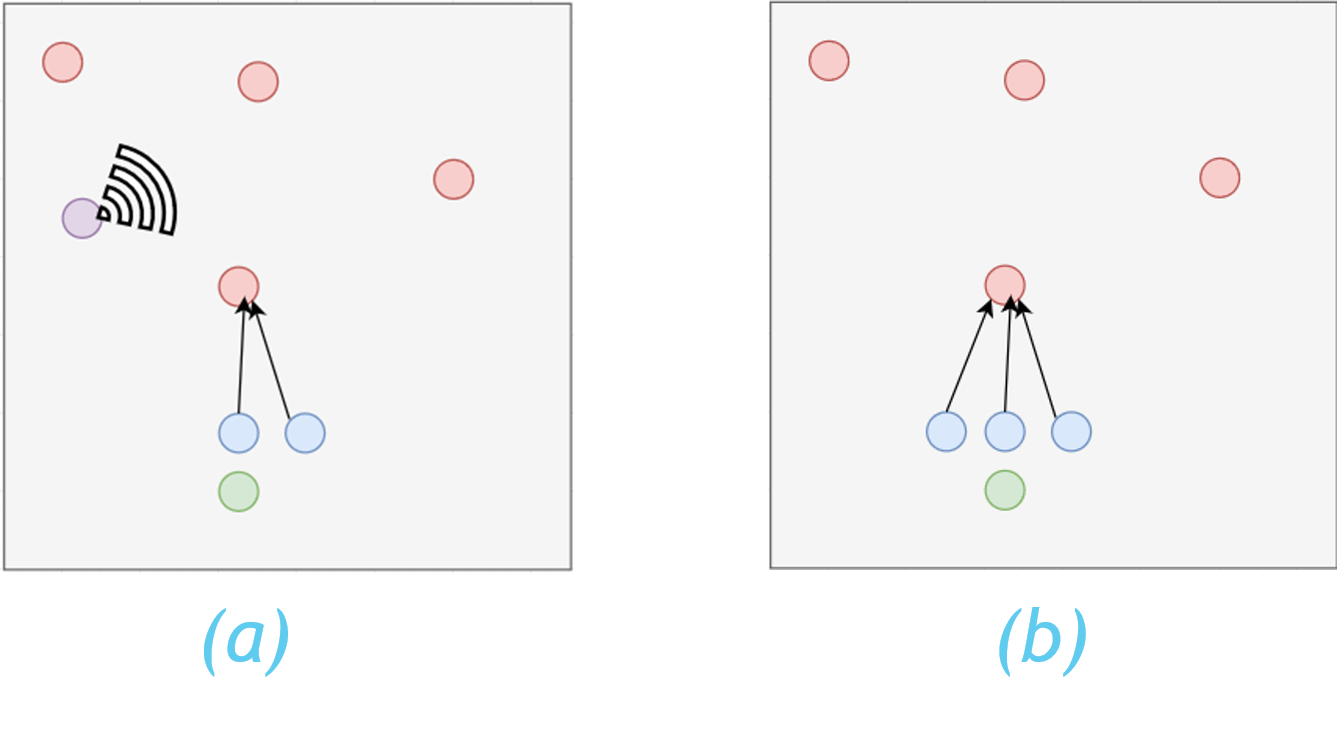
\includegraphics[scale=0.4]{Imagens/Imagem2.png}
    \caption{Esquema (a) Exemplo do Scanning do robot \textit{Seeker} e atribuição de ordens aos robots \textit{Destroyers}; (b) Exemplo do ataque dos robots \textit{Destroyers} após receberem ordens do robot \textit{Seeker}.}
    \label{fig:tact1}
\end{figure}

\begin{figure}[H]
    \centering
    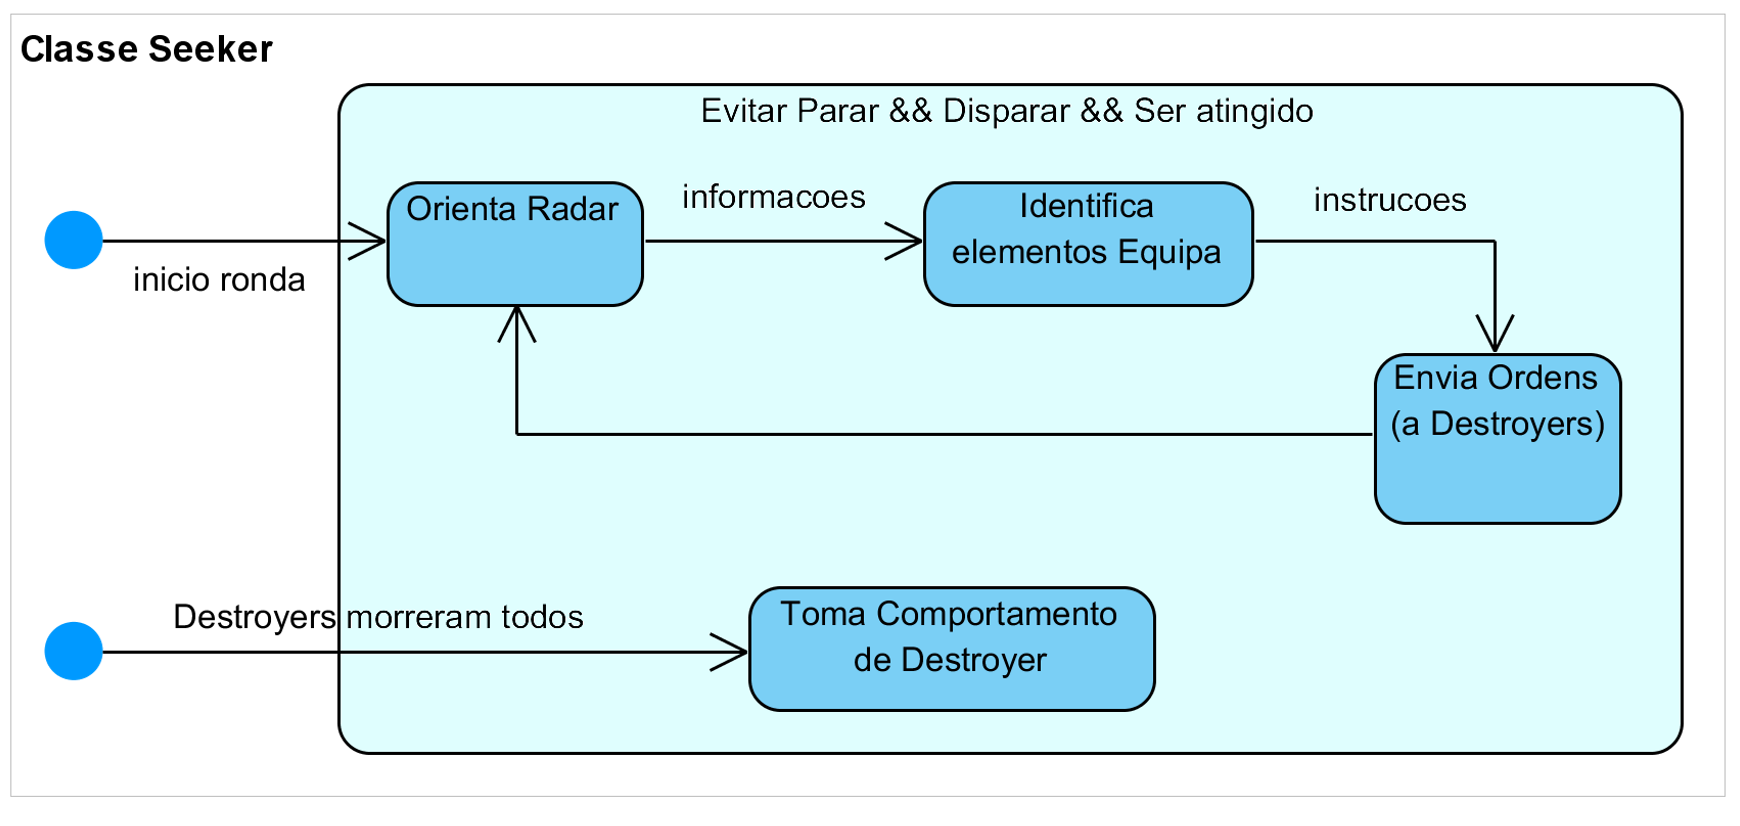
\includegraphics[scale=0.5]{Imagens/evt1.png}
    \label{fig:evet1}
    
    \centering
    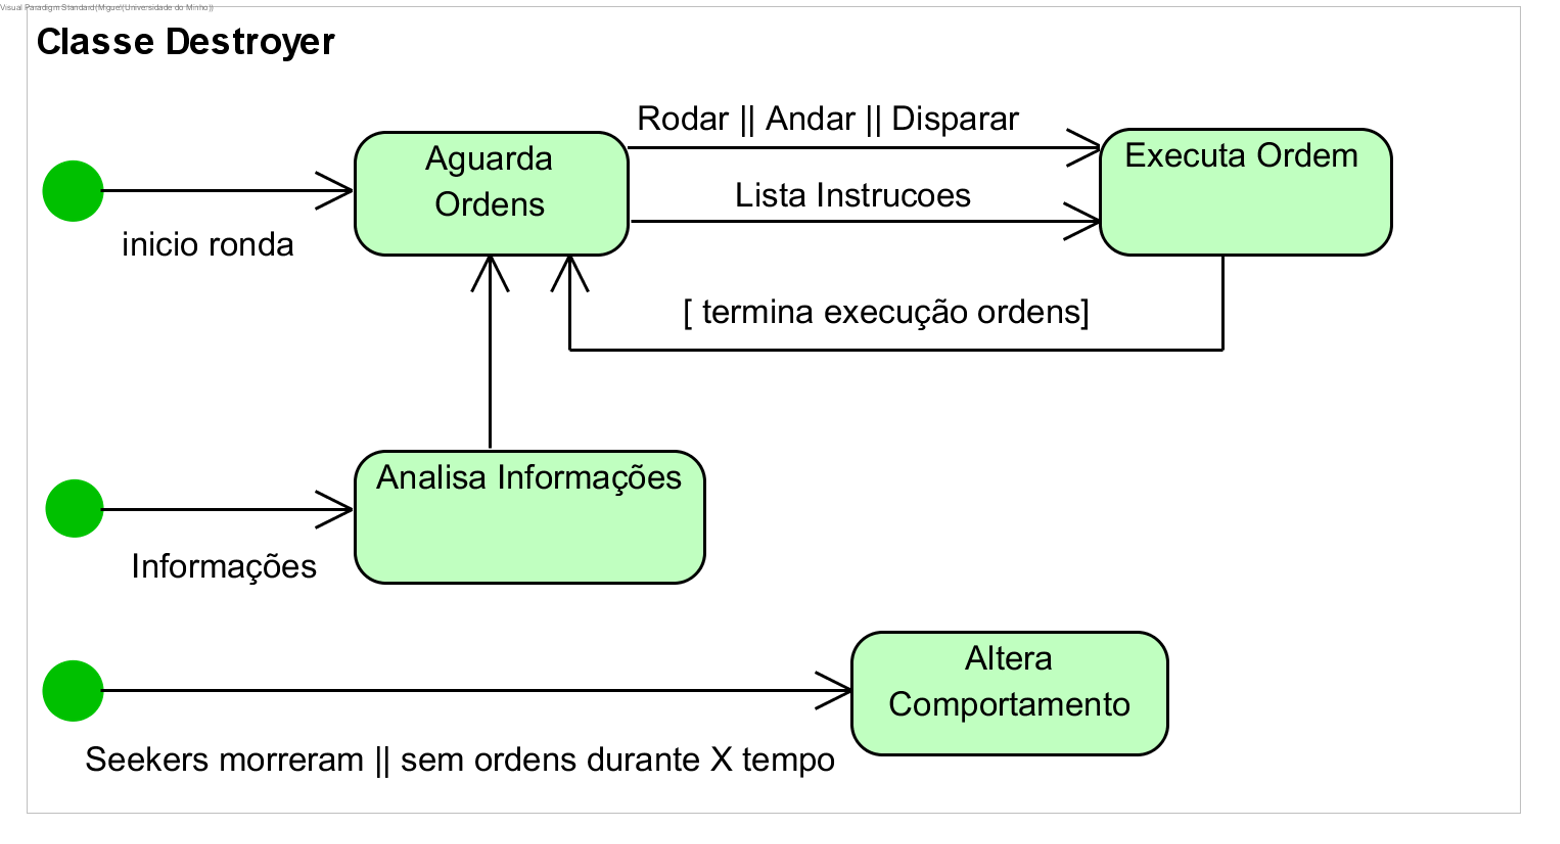
\includegraphics[scale=0.5]{Imagens/evt2.png}
    \caption{Esquema do conjunto de eventos que alteram o estado/comportamento emocional do robot \textit{Seeker} e \textit{Destroyer}.}
    \label{fig:evet2}
\end{figure}
\newpage


Relativamente ao comportamentos dos robots \textit{Destroyer}:
\begin{itemize}
    \item Este tipo de \textit{robots} têm por base a classe \textit{Droid} existente na plataforma \textit{RoboCode}. 
    
    Pela sua simplicidade, estes robots não possuem radares ou qualquer tipo de sensorização do ambiente ou dos robots existentes no ambiente onde se insere.
    Desta forma, as suas ações e tomadas de decisão dependem exclusivamente das informações e instruções recebidas por mensagem por parte do Seeker (chefe) da sua equipa;
    
    \item O seu comportamento é manifestado através das ações que realiza. 
    As ordens recebidas pelo \textit{Seeker} podem ser simples ou pedidos executar uma sequência de instruções;
    
    Ordens simples caracterizam instruções para rodar o robot, deslocar-se, disparar ou atualizar as informações sobre inimigos e pontos do campo de batalha a evitar. 
    Sequências de instruções apresem uma lista com um conjunto das ações anteriormente citadas. 

    \item Se o \textit{Seeker} da equipa for eliminado/destruído, os robots que sigam a classe \textit{Destroyers} deixam de receber ordens que permitam o sucesso global da equipa. 
    
    Assim, como forma de evitar que os mesmos fiquem parados no campo de batalha, os robots apresentam a capacidade de alterar o seu comportamento. Esta mudança ocorre quando deixam de receber ordens do robot líder durante um determinado período de tempo ou, quando verificam que a energia do \textit{Seeker} se encontra bastante baixa. 
    
    A alteração de comportamento passa por assumir um comportamento mais reativo face aos inimigos restantes.
\end{itemize}


\chapter{Código implementado}

\section{Classes Auxiliares}

As classes criadas são as seguintes:

\begin{itemize}
    \item \textit{\textbf{Accuracy}} - Classe responsável por armazenar a informação sobre as trajetórias inimigas.
    
    Supondo o normal funcionamento da equipa, os robots \textit{Destroyers} são os únicos a realizar ataques à equipa inimiga. 
    Para desempenhar esta tarefa, os \textit{Destroyers} recebem ordens para atacar um determinado inimigo, escolhendo 1 de 3 métodos implementados para o cálculo da trajetória de disparo. 

    À medida que o jogo se desenvolve, são guardados registos de cada disparo de forma a que, num disparo futuro, se observe a média de \textit{accuracy} que cada algoritmo obtém num determinado contexto com o robot inimigo.  
    Cada método/algoritmo de previsão de movimentos/trajetória assume três cenários: o inimigo pode deslocar-se linearmente, em círculos ou estar imóvel, num estado estacionário.
    
    
    \item \textit{\textbf{CircularIntercept}} - Esta classe invoca métodos que realizam a atualização da previsão da posição de um robot inimigo. 
    
    A classe estende a classe \textit{Intecept} e, tal como o nome indica, é utilizada para definir que a previsão da posição do robot inimigo assume um movimento circular do mesmo, em vez de um movimento linear. 
    
    Assim, para calcular qual a direção sobre a qual realizar um disparo, assume-se que o inimigo está a deslocar-se num percurso circular. 
    
    \item \textit{\textbf{Coordinate}} - Classe criada para representar um ponto com coordenadas X,Y. 
    
    Estas coordenadas são posteriormente utilizadas para identificar objetos, pontos a evitar ou inimigos dentro das dimensões do campo de batalha. 
    
    \item \textit{\textbf{Gravity}} - Classe utilizada para implementar o algoritmo de \textit{Anti-Gravity Movement}. 
    
    A tática implementada nesta classe permite calcular as trajetórias que cada robot deve seguir ao longo do decorrer de uma \textit{round} de um jogo;
    
    \item \textit{\textbf{Intercept}} - Classe responsável por calcular a previsão das próximas coordenadas de um robot.
    
    Para isso, os métodos têm por base a posição inicial/atual do robot, a sua direção e a velocidade, selecionando um possível tipo de trajetória (movimento linear, circular ou estacionário), calcula com os parâmetros citados a nova posição do robot;
    
    \item \textit{\textbf{Order}} - Implementação que representa uma ordem/instrução enviada do \textit{Seeker} para os \textit{Destroyers}.
    
    Esta classe possui informações sobre o tipo da ordem disparar, andar, rodar, atualizar informações sobre as coordenadas para as quais disparar, coordenadas para as quais nos devemos deslocar e ângulos a rodar
    
    \item \textit{\textit{Orders}} - Classe simples que implementa uma abstração de uma lista de ordens, de forma a enviar várias ordens ao mesmo tempo aos \textit{Destroyers};
    
    \item \textit{\textbf{Point}} - Classe semelhante à \textit{Coordinate}. 
    Além de guardar as coordenadas (X,Y) de um ponto, tem também o seu "poder" de atração, de forma a implementar os conceitos da tática "Anti-Gravity". 
    
    Se o poder de atração de uma determinada coordenada for positivo é um ponto atrator, se for um ponto negativo representa um ponto repulsor. Estas coordenadas podem representar um inimigo ou elementos da própria equipa; 
    
    \item \textit{\textbf{State}} - Estado lido a partir de um \textit{robot}, contem todas as informações lidas pelo scanner e a posição onde foi encontrado o robot em questão;
    
    \item TeamInfo - Contem o estado atual do jogo, desde pontos de gravidade, inimigos, membros da equipa e os respetivos estados e  o robot inimigo prioritário a abater;
\end{itemize}


\section{Classes Principais}

Neste projeto definimos que a nossa equipa iria ser constituída por dois tipos de robots, um deles seria o líder da equipa equipado com um radar para que possa conhecer o estado do jogo e informar o resto da equipa e o outro seria um \textit{droid}, que tem a vantagem de ter mais 20 pontos de energia, porem, não tem radar e depende de um líder para lhe indicar o que fazer.

Alem do comportamento enunciado em baixo os dois robots tem tambem alguns pontos em comum, como funções que são ativadas por eventos, como \textit{onHitWall()} e \textit{onHitByBullet()}, que nestes casos executam pequenas tarefas como mudar o seu ângulo ou movimentar se um pouco de forma a corrigir alguns comportamentos do algoritmo principal de deslocamento.

\subsection{Droid - Destroyer}

O \textit{Destroyer} é o robot com comportamento mais simples. Este aplica o algoritmo de \textit{Anti-Gravity Movement} para evitar deslocar-se pelo terreno de jogo enquanto espera por mensagens do seu líder. As mensagens podem conter o estado atual do jogo de forma a que o robot se atualize, ou uma lista de ordens a serem executadas sequencialmente, sendo que cada ordem pode consistir num disparo, num deslocamento ou mudar o ângulo do robot. 
No caso de o \textit{Seeker} ficar com 0 energia, este robot deixa de receber ordens e portanto apenas continua com o seu movimento de forma a evitar ser atingido por balas inimigas, na esperança que os restantes robots se destruam quer por passar do tempo de jogo, quer por balas enviadas pelos membros da própria equipa ou até por colisões contra outros robots e paredes.

\subsection{Lider - Seeker}
O robot Seeker tem muito em comum com o \textit{Destroyer}, usa o mesmo algoritmo para efetuar movimento, mas em vez de esperar por mensagens, este é o responsável por las enviar, assim sendo, é de máxima importância que este permaneça vivo a ronda toda. Assim sendo este robot não dispara a não ser em casos extremos, como por exemplo a restante equipa já estar toda com 0 pontos de energia e os inimigos terem mais energia do que os aliados, se estas duas condições não se reunirem simultaneamente, o robot não dispara.

Ao mesmo tempo que o robot percorre o terreno roda o seu radar 360 graus por cada ronda, sendo que sempre que avistar um robot avalia se este pertence à sua equipa ou não, atualiza o estado de jogo, envia o estado de jogo a todos os robots e além disso se confirmar que encontrou um robot da outra equipa envia também  a ordem de disparo aos \textit{Droids} para que estes tentem atingir o robot em questão.




\section{Algoritmos principais}

\subsection{Anti-Gravity Movement}
Este algoritmo é baseado na criação de pontos que vão representar forças que ao serem aplicadas no nosso robot iram fazer com que este se desloque ate outro ponto.

Os pontos são criados com base na posição dos outros robots de forma a que os outros robots exerçam uma força repulsiva no robot em questão evitando assim colisões.

Por exemplo:

\begin{figure}[H]
    \centering
    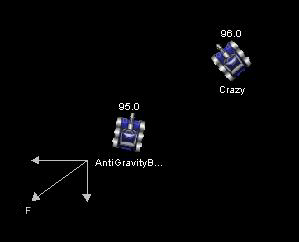
\includegraphics[scale=0.6]{Imagens/force.png}
    \caption{Esquema de forças causadas por 1 robô.}
    \label{fig:forca}
\end{figure}

Neste exemplo temos dois robots, em que o robot \textit{Crazy} executa a força F no robot \textit{AntiGravityBot}, esta força é representada por um componente em X e outro em Y.

A soma de todas as forças causadas por todos os robots irá criar a direção para a qual o robot tem de se deslocar.

Este algoritmo pode causar problemas como por exemplo, se os robots estiverem todos a direita do robot em questão, este irá ser enviado para a parede esquerda do tabuleiro e ficar preso contra a parede, para combater este problema criaram se pontos de repulsão ao longo das 4 paredes do tabuleiro desta forma combatemos o problema de ele ficar preso contra uma parede.

Alem dos pontos de repulsão criados pelas bordas e pelos robots a cada iteração deste algoritmo são definidos alguns pontos com coordenadas aleatórios, mas desta vez com forças positivas, ou seja pontos atratores, são estes pontos que iram tornar o algoritmo menos previsível e fazer com que todos os robots tenham trajetórias diferentes.

Como melhorias a este algoritmo podem ser alterados alguns parâmetros relativos as forças tais como elevar as forças a um parâmetros N e variar esse parâmetro, podemos adicionar pontos ou igualar as forças dos pontos de forma a termos um resultado mais consistente.

\subsection{Predictiv Targeting}

Para aproveitar ao máximo a energia disparada pelos robots, foi criado um método que prevê onde é que os robots irão estar nos momentos seguintes. 

Esta algoritmo tem capacidade para prever 3 situações: a primeira e mais simples é o caso do robot em questão não se mexer, ou seja se ele não se mexer a sua posição será no mesmo ponto onde foi encontrado.

Temos também um método que assume que o movimento do robot é retilíneo e uniforme e assim sendo sabendo a posição inicial do robot, a sua direção e velocidade conseguimos prever a sua próxima posição. 

Por fim, temos um terceiro método que assume que o movimento do robot é curvilíneo e tenta encontrar a posição onde o robot se irá encontrar partindo dessa assunção.

Inicialmente o robot começa por usar o algoritmo linear já que este foi considerado o caso mais comum, se este falhar testa se método de disparo para o sitio onde o robot foi encontrado e por fim, se este se mostrar pouco eficiente testa o algoritmo curvilíneo.
\chapter{Conclusão e Trabalho Futuro}
\label{chp:conclusao}

Depois de analisados e descritos os princípios e algumas metodologias Ágeis, constata-se que estas trouxeram melhorias notórias nos processos e fluxos de trabalho das empresas, que se convertem em maior organização, capacidade de produção e consequentemente, satisfação dos clientes. É de notar também que, apesar do que muitas pessoas possam imaginar, estas metodologias não são propriamente recentes. Já foram inventadas há alguns anos, mas só começaram a popularizar-se na área da produção de Software há relativamente pouco tempo e o seu uso tem vindo a tornar-se cada vez mais comum. Apesar das vantagens das abordagens mais Ágeis, elas têm vantagens e desvantagens e não servem para todo o tipo de projeto.\\
Na nossa opinião o método desenvolvido tem algumas características que à partida definimos como prioritárias: é simples, não demora muito a responder, é direto e ajuda a ter uma primeira perceção do método de trabalho a seguir.\\
É também importante definir que esta é apenas uma primeira versão do método de diagnóstico, será esperado que como trabalho futuro se sugira uma segunda parte do questionário que apenas seja respondida se a primeira parte indicar que o projeto deva seguir uma abordagem ágil, e onde se consiga perceber em específico que método Ágil o projeto deve seguir. Para além disso, e devido ao facto de o desenvolvimento deste projeto ter sido feito num contexto académico com prazos limitados, é também importante validar as questões num contexto real em projetos já desenvolvidos e onde se consiga ter uma perceção se as abordagens ágeis ou tradicionais resultaram.

\bibliographystyle{unsrt}
\chapter{Bibliografia}

\url{https://www.ibm.com/developerworks/library/j-robotips}


\url{https://www.ibm.com/developerworks/library/j-tipstrats/index.html}

\end{document}